\subsection{Load following}
\begin{frame}
\frametitle{Why load following nuclear reactor is a game changer?}
	\begin{textblock*}{12.1cm}(0.3cm,1.65cm) % {block width} (coords)
\begin{figure}[t]
	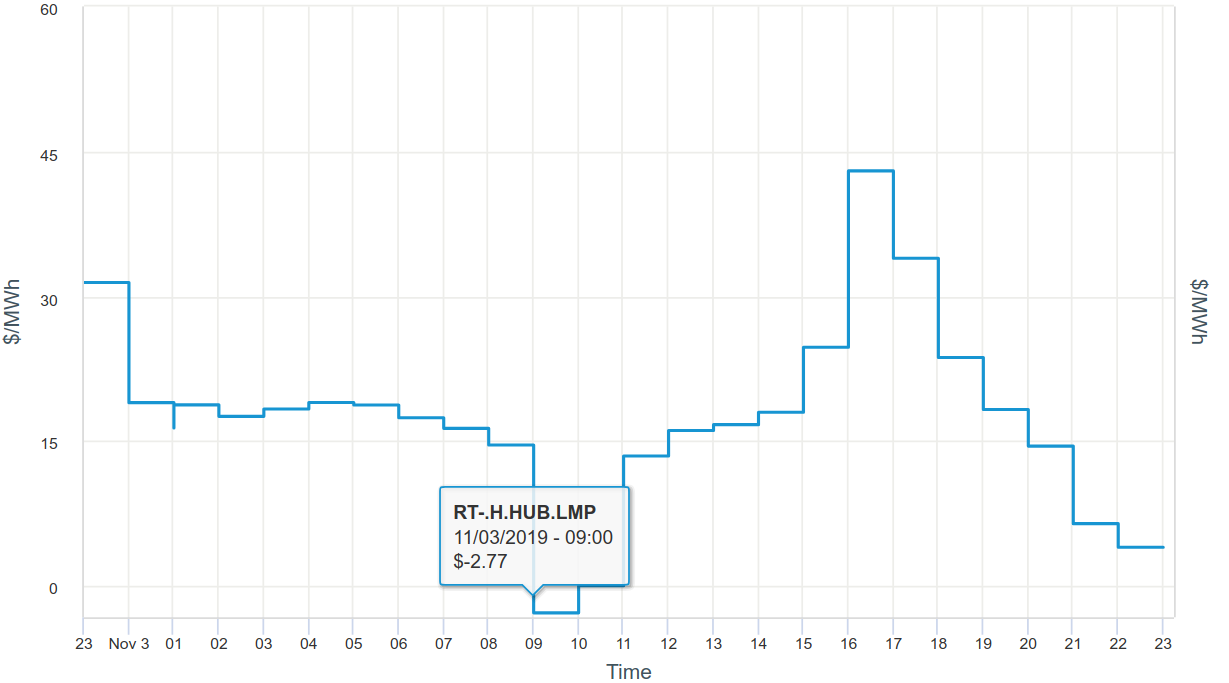
\includegraphics[width=\textwidth]{./images/ne_one_day_price.png}
		\vspace{-6mm}
	\caption{ISO New England hourly electricity price; November 3, 2019 
	from 00:00AM to 11:00PM (Source: https://www.iso-ne.com/).}
\end{figure}  
\end{textblock*}
\end{frame}

\begin{frame}
\frametitle{Nuclear Power Plants as a based-load vs load-following}
	\vspace{-4mm}
\begin{overlayarea}{\linewidth}{20\baselineskip}
	\begin{block}{Historically used as base-load source of electricity}<1->
		\begin{enumerate}
			\item Usually simplier and more efficient
			\item Nuclear fraction in total power generation was small
			\item Maneuvering capabilities limited to frequency regulation
		\end{enumerate}
	\end{block}
	\begin{block}{Motivation for load-following with nuclear power}<2->
	\begin{enumerate}
		\item The share of nuclear power in total generation became large 
		(75\% in France)
		\item Large-scale deployment of intermittent renewables (wind, solar)
	\end{enumerate}
	\end{block}
	\begin{block}{Physical effects limiting the maneuvering capabilities 
		\cite{lokhov_technical_2011}}<3->
	\begin{enumerate}
		\item<3-> Moderator effect (primary coolant temperature change)
		\item<3-> Doppler effect (fuel temperature change)
		\item<4-> Fuel burnup (low excess of reactivity at EOC)
		\item<5-> \textbf{Xenon-135 poisoning (iodine pit)}
	\end{enumerate}
\end{block}
\end{overlayarea}
\end{frame}

\begin{frame}
\frametitle{What is Xenon-135 poisoning?}
\animategraphics[loop,controls,width=1.07\linewidth]{0.5}{./images/anime/xe_pois-}{0}{11}
\end{frame}

\subsection{Molten Salt Reactors}

\begin{frame}
\frametitle{Potential Generation IV reactor systems \cite{abram_generation-iv_2008}}
\begin{figure}[t]
	\vspace*{-0.1in}
	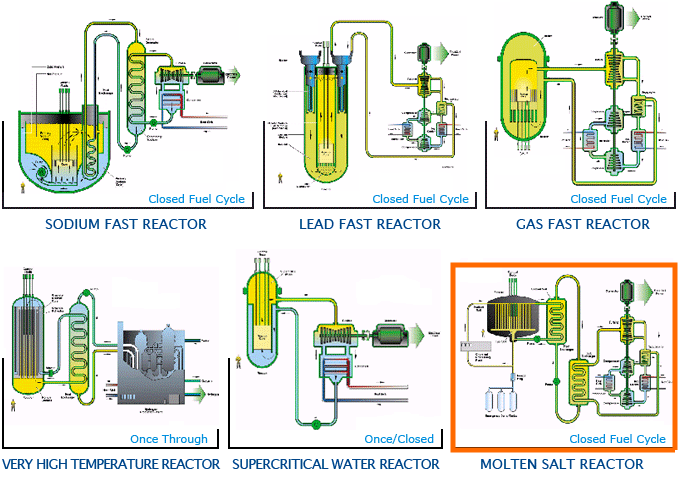
\includegraphics[height=0.7\textwidth]{./images/6_types.png}
	\caption{\gls{MSR} design}
\end{figure}            
\end{frame}


\begin{frame}
\frametitle{MSR (Molten Salt Reactor) types}
\begin{overlayarea}{\linewidth}{20\baselineskip}
\begin{block}{Stationary Fuel}<1-4>
	\begin{enumerate}
		\item Graphite block with TRISO fuel, clean salt works as 
		coolant (Fluoride-Salt-Cooled High-Temperature 
		Reactor (FHR))
		\item Plate Fuel: hexagonal fuel assembly is similar in shape to a typical sodium-cooled reactor
		\item Fuel Inside Radial Moderator (FIRM)
		\item Liquid fuel salt inside fuel rods cooled by clean salt 
		(Moltex Stable Salt Reactor)
	\end{enumerate}
\end{block}

\begin{block}{Mobile Fuel}<2-4>
	\begin{enumerate}
		\item<2-4> Mobile solid fuel elements (pebbles) cooled by 
		clean salt (PB-FHR)
		\item<3-4> Non-circulating liquid fuel salt (TerraPower \gls{MCFR}) 
		\item<4> \textbf{Circulating liquid fuel salt} which also works 
		as coolant (\gls{MSBR})
	\end{enumerate}
\end{block}
\end{overlayarea}
\end{frame}


%\begin{frame}
%\frametitle{Stationary and Mobile Solid fuel}
%\vspace*{-0.1in}
%\begin{figure}[t]
%	\hspace*{-0.35in}
%	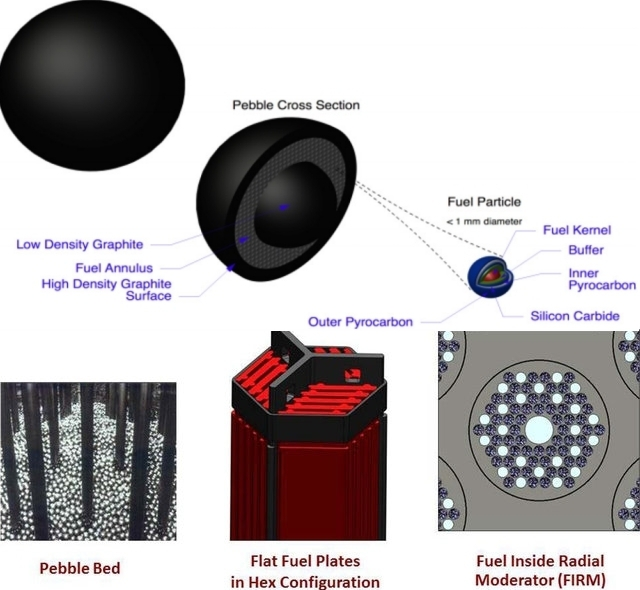
\includegraphics[height=0.63\textwidth]{./images/solid_fuel.jpg}
%	\caption{TRISO fuel particle (top) and FHR fuel designs (bottom) 
%	\cite{forsberg_basis_2016}.} 
%\end{figure}   
%\end{frame}

\begin{frame}
\frametitle{Mobile, Non-Circulating, Liquid Fuel}
\begin{figure}[t]
\vspace*{-0.1in}
\hspace*{-0.35in}
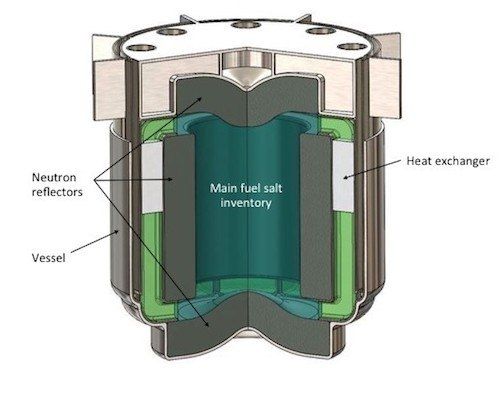
\includegraphics[height=0.6\textwidth]{./images/mcfr-crossection.jpg}
\caption{The TerraPower MCFR is an example of reactor design with 
\textbf{liquid, mobile, non-circulating} chloride salt fuel 
\cite{doene_southern_2018}.}
\end{figure}   

\end{frame}


\begin{frame} % Add another slide with red rectangular around reprocessing system
\frametitle{Mobile, Circulating, Liquid Fuel}
\vspace{-2mm}
\begin{figure}[t]
      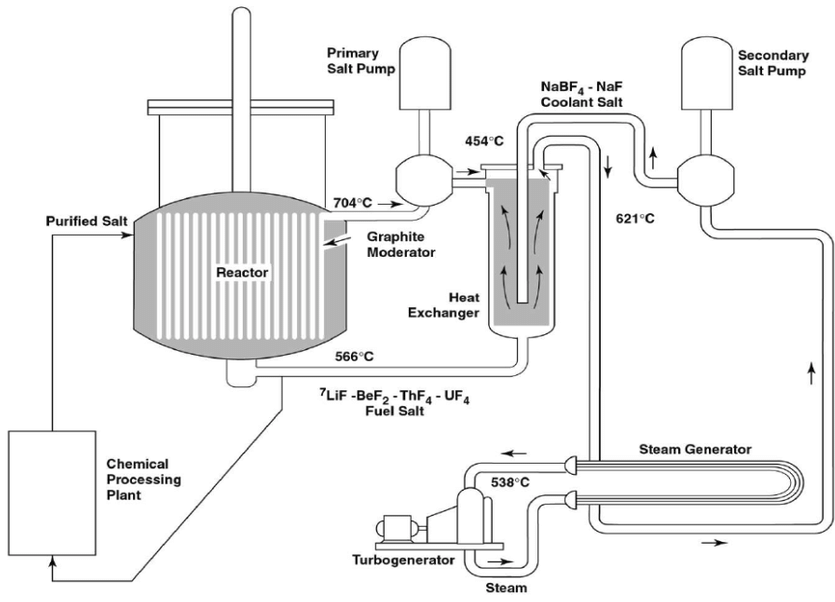
\includegraphics[height=0.6\textwidth]{./images/msbr_scheme.png}
	\caption{The \gls{MSBR} is an example of reactor design with 
	\textbf{liquid, mobile, circulating} fluoride salt fuel 
	(reproduced from Rosenthal \emph{et al.} 
	\cite{rosenthal_molten-salt_1970}).}
\end{figure}   

\end{frame}


\subsection{Motivation}

\begin{frame}
\frametitle{Why Molten Salt Reactors with circulating fuel?}
\begin{block}{Liquid-fueled \gls{MSR} designs have following \textbf{potential} advantages:}
	\begin{enumerate}
		\itemsep1em
		\item High coolant temperature (600-750$^{\circ}$C) 
		$\Rightarrow$ potentially high thermal efficiency, process 
		heat for chemical industry
		\item Fuel diversity ($^{235}$U, $^{233}$U, Thorium, U/Pu)
		\item Strong negative fuel temperature feedback 
		\item Passive safety $\Rightarrow$ fuel drains into tanks 
		in emergency
		\item High fuel utilization $\Rightarrow$ reduced spent fuel 
		generation
		\item<2> \textbf{On-line (continuous) fuel reprocessing potentially  
		helps to reduce Xenon-135 poisoning} $\Rightarrow$ more flexible  
		power maneuvering
	\end{enumerate}
\end{block}

\end{frame}


\subsection{Research objectives}

\begin{frame}
  \frametitle{Research objectives of this work}
     Analyze the \glsfirst{TAP} \glsfirst{MSR} neutronic performance during 
     load following at the \glsfirst{BOL} and inactive online fission products 
     removal system.
  \begin{overlayarea}{\linewidth}{20\baselineskip}
     \begin{block}{Goals of current study}<1->
         \begin{enumerate}
         		\itemsep1em
                \item<1-> Create high-fidelity full-core 3-D model of 
                \glsfirst{TAP} \glsfirst{MSR}, without any
approximations 
                using Serpent 
                \cite{leppanen_serpent_2014}
                \item<2-> Perform fuel salt depletion to study 
                \textbf{$^{135}$Xe/$^{135}$I balance dynamics during 
                load-following}
            	\item<3-> Analyze $k_{eff}$ dynamics during this transient 
                \item<4-> Compare obtained results with well-studied 
                \glsfirst{PWR} behavior
         \end{enumerate}
      \end{block}
  \end{overlayarea}
\end{frame}
